
\documentclass{sig-alternate-05-2015}
\usepackage{textcomp}
\usepackage{amsmath}
\usepackage{algpseudocode}
\newcommand{\pluseq}{\mathrel{+}=}

\begin{document}

% Copyright
\setcopyright{acmcopyright}
%\setcopyright{acmlicensed}
%\setcopyright{rightsretained}
%\setcopyright{usgov}
%\setcopyright{usgovmixed}
%\setcopyright{cagov}
%\setcopyright{cagovmixed}


% DOI
\doi{December 12, 2016}

% ISBN
%\isbn{Fall 2016 UW Madison}

%Conference
\conferenceinfo{CS838 Fall 2016}{University of Wisconsin-Madison}

%\acmPrice{\$15.00}

%
% --- Author Metadata here ---
%\conferenceinfo{WOODSTOCK}{'97 El Paso, Texas USA}
%\CopyrightYear{2007} % Allows default copyright year (20XX) to be over-ridden - IF NEED BE.
%\crdata{0-12345-67-8/90/01}  % Allows default copyright data (0-89791-88-6/97/05) to be over-ridden - IF NEED BE.
% --- End of Author Metadata ---

\title{Geo Distributed Storage using EC - Measurements \& Improvements}
\subtitle{CS838 Fall 2016 Project Report}
%
% You need the command \numberofauthors to handle the 'placement
% and alignment' of the authors beneath the title.
%
% For aesthetic reasons, we recommend 'three authors at a time'
% i.e. three 'name/affiliation blocks' be placed beneath the title.
%
% NOTE: You are NOT restricted in how many 'rows' of
% "name/affiliations" may appear. We just ask that you restrict
% the number of 'columns' to three.
%
% Because of the available 'opening page real-estate'
% we ask you to refrain from putting more than six authors
% (two rows with three columns) beneath the article title.
% More than six makes the first-page appear very cluttered indeed.
%
% Use the \alignauthor commands to handle the names
% and affiliations for an 'aesthetic maximum' of six authors.
% Add names, affiliations, addresses for
% the seventh etc. author(s) as the argument for the
% \additionalauthors command.
% These 'additional authors' will be output/set for you
% without further effort on your part as the last section in
% the body of your article BEFORE References or any Appendices.

\numberofauthors{2} %  in this sample file, there are a *total*
% of EIGHT authors. SIX appear on the 'first-page' (for formatting
% reasons) and the remaining two appear in the \additionalauthors section.
%
\author{
% You can go ahead and credit any number of authors here,
% e.g. one 'row of three' or two rows (consisting of one row of three
% and a second row of one, two or three).
%
% The command \alignauthor (no curly braces needed) should
% precede each author name, affiliation/snail-mail address and
% e-mail address. Additionally, tag each line of
% affiliation/address with \affaddr, and tag the
% e-mail address with \email.
%
% 1st. author
\alignauthor
Karan Bavishi \\
       \affaddr{UW Madison}\\
% 2nd. author
\alignauthor
Hasnain Ali Pirzada\\
\affaddr{UW Madison}\\
% 3rd. author
}


\maketitle
\section{Problem Statement}
HDFS and other distributed file systems do not scale well to geo distributed environments. The primary reason is that these file systems are unaware of the heterogeneity in speeds of the the inter and intra datacenter links.

There have been several solutions in this problem space, which focus on query optimization, task placement and data movement using WAN awareness to reduce WAN link usage and achieve better performance.  We take a significantly different approach to solving this problem, i.e we focus on whether using Erasure Coding (EC) instead of replication can result in better solutions. Using EC results in much lesser data overhead compared to replication. This can reduce the amount of data sent on WAN links and also result in storage efficient solutions.

Our goals in this project were two fold. Our first target was to quantify and analyze the performance degradation of HDFS when run in a geo-distributed setting naively, using both replication and EC. Our second major goal was to come up with measures to improve the performance of naive HDFS-EC by accounting for the presence of thin WAN links.

We achieved these goals by first benchmarking both HDFS and HDFS-EC in a geo distributed setting and comparing their performance to a single datacenter setting. In the second phase of the project we have modified HDFS-EC and used greedy heuristics to make it WAN aware in both its reads and writes.

\printccsdesc


\keywords{HDFS; Erasure Coding; Geo Distributed Storage}

\section{Erasure Coding Overview}
In this section, we provide an overview of erasure coding and its availability as an inbuilt feature in HDFS 3.0.0. We also briefly discuss its performance in comparison to the replica-based fault tolerance scheme which is used by default.

\subsection{Basics}
The \emph{Reed-Solomon (RS)} family of erasure codes has become a widely used redundancy scheme in many production datacenters owing to its storage benefits. In all RS(n, k) codes, we have \emph{k} parity chunks for each \emph{n} chunks of data. This results in a storage overhead of \( \frac{n+k}{n} \).  

Commonly employed RS schemes include RS(10,4) and RS(6,3) which result in storage overheads of $1.4\times $ and $1.5\times $ respectively. This overhead is a significant improvement on the overhead of $3\times $ incurred by using the replica-based redundancy scheme

For a read operation, any \emph{n} chunks from the \emph{n+k} can be fetched to generate the data. Most systems prefer to fetch \emph{n} data chunks so that no extra computation is required. In case some chunks are lost, the required number of parity chunks are fetched and RS decoding is employed to generate the data.

\subsection{Erasure Coding in Hadoop}
Hadoop now includes support for online erasure coding in its \emph{3.0.0-alpha1} release\cite{hdfs-ec}. It allows for the encoding \& decoding in an online manner, i.e. during the read \& write operations. This provides us significantly more flexibility over the original HDFS-RAID\cite{hdfs-raid} implementation, which does erasure coding as a periodic background task.

\subsection{Comparison with replica-based HDFS}
It is commonly believed that using erasure coding results in a significant performance penalty. However, we observe that HDFS-EC equals, and in some cases outperforms, the replica-based HDFS in terms of the observed read and write throughputs. These findings are discussed in more detail in Section \ref{sec:bench-results}, and are consistent with findings made in previous studies\cite{cloudera-blog}.

Much of the improved performance results from the use of Intel's ISA-L libraries\cite{isa-l}. These libraries provide support for fast encoding/decoding for RS codes, by using hand-written assembly codes which use the underlying AVX and AVX2 features of the Intel architectures.

\section{System Design \& Implementation}
Based on the results discussed in Section \ref{sec:bench-results}, we find that the performance of HDFS-EC can be severely impacted, if deployed naively in a geo-distributed (GD) setting without link cost awareness. 

Drawing insights from these results, we implemented support for WAN awareness in HDFS-EC, which allow for the selection of datanodes based on their link speeds. We added support for both the read and write pipelines, and thus improve performance considerably. 

\begin{figure}
\centering
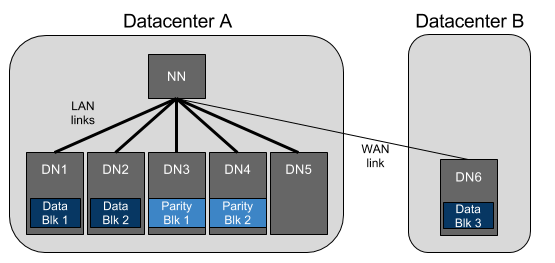
\includegraphics[scale=0.45]{gda_diagram_2.png}
\caption{An example geo-distributed topology which uses HDFS-EC with RS(3,2). Thick lines represent high-speed LAN links. Thin lines represent low-speed WAN links.}
\label{gda-topo}
\end{figure} 

\subsection{WAN awareness for EC Reads with Greedy Heuristics}
\textbf{Motivation:} We build the motivation for the need of WAN awareness in EC reads with an example. Consider the topology described in Figure \ref{gda-topo}, which uses the RS(3,2) scheme to store data. It contains the data \& parity blocks for a particular file, such that datacenter A hosts 2 data and 2 parity blocks whereas datacenter B hosts 1 data block.

Now, assume that there is a client in datacenter A which wants to read that file. The default policy is to fetch all the data blocks and to avoid parity blocks because of the high computation cost of reconstructing the data. This policy makes sense in non-GD settings, where the computation cost is very likely to exceed the network cost of fetching the data blocks.  However in a GD cluster, this may not be true because the WAN link speed is much lower than that of intra DC links. In our example, it might be faster to fetch the parity blocks from A and reconstruct the data, rather than fetching the data block residing in datacenter B over the slow WAN link.

\textbf{Greedy heuristics:} To achieve this, we first imbibe link cost awareness into HDFS. This is done by modifying the namenode behaviour to call a \emph{link awareness} script when datanode registration happens. This script allows the namenode to be aware of the link cost between any two pair of datanodes using their rack locations. In our current model, the costs are static and hardcoded in our script. 

After this, we build a greedy approach for picking EC chunks based on their costs. A simplified version in pseudocode is described below:
\vspace{0.5em}
\begin{algorithmic}
\Function{pickChunksGreedy}{n, client, chunks} 
\For {chunk i in chunks}
\State $cost[i]\gets \Call{linkCost}{client.rack, chunk[i].rack}$
\If {chunk[i].isParity}
    \State $cost[i]\gets cost[i] + computationPenalty$
\EndIf
\EndFor

sortedChunks = \Call{sortChunksByCost}{chunks, cost}

\Return sortedChunks[:n]
\EndFunction
\end{algorithmic}
\vspace{0.5em}

The \emph{pickChunksGreedy} function is called for every erasure-coded stripe in a file. It basically picks \emph{n} chunks (or stripe units) out of a possible \emph{n+k} chunks in an RS(n,k) scheme, in a greedy manner. The cost associated with each chunk equals the link cost from the client to the datanode hosting the chunk. Parity chunks incur an additional penalty called \emph{computationPenalty} because of the computational costs associated with reconstruction. The \emph{computationPenalty} can be configured through an HDFS config knob.

So in our earlier example, if we keep the WAN costs to be higher than the \emph{computationPenalty}, the client would read 2 data cells and 1 parity cell from datacenter A and use these to reconstruct the data.

\subsection{WAN awareness for EC Writes with Greedy Heuristics}
During HDFS-EC writes, the namenode selects \emph{n+k} datanodes to host data and parity cells in an RS(n,k) scheme. In order to provide greater fault tolerance to rack power failures, the namenode tries to select datanodes across multiple racks. 

However this behaviour of picking multiple racks can result in the data being spread across multiple datacenters in a GD setting. An example of this can be seen in Figure \ref{gda-topo}. In order to achieve good performance in such a case, we must incur the extra computation overhead associated with fetching the local parity chunks.

In cases like these, it may make sense to sacrifice rack fault tolerance for better performance. In our example topology, it might be better to pick the 5 datanodes hosted at datacenter A while creating the file. 

\textbf{Greedy heuristics:} We again build a greedy approach for picking the datanodes for hosting the blocks during file writes, which tries to balance rack fault tolerance along with the link costs associated with the datanodes. A simplified version is described in pseudocode below:

\vspace{0.5em}
\begin{algorithmic}
\Function{selectDatanodesGreedy}{n, client, racks} 
\For {rack i in racks}
  \State $cost[i]\gets \Call{linkCost}{client.rack, rack[i]}$
\EndFor

rackHeap = \Call{sortRacksByCost}{racks, cost} 
\\
\State $chosenDatanodes \gets []$

\While {$chosenDatanodes.size() < n$} 
  \State $bestRack, cost\gets rackHeap.min()$
  \State $chosenDatanodes \pluseq bestRack.getRandomDatanode()$
  \If {$bestRack.datanodes.size() > 0$}
      \State $cost \gets cost + sameRackPenalty$
      \State rackHeap.addEntry(bestRack, cost)
  \EndIf 
\EndWhile

\Return chosenDatanodes
\EndFunction
\end{algorithmic}

\vspace{0.5em}
This function \emph{selectDatanodesGreedy} is invoked every time a new block is to be created, and helps select the datanodes to host the data and parity cells for the new block. The function first builds a heap of racks, arranged by their link costs. It then picks the rack with the lowest cost, and picks a random datanode from that rack. If the rack contains more datanodes, it is re-inserted into the heap but with an additional penalty called the \emph{sameRackPenalty}. This penalty allows us to balance the goals of rack fault tolerance with link costs. Its value is configurable through an HDFS config knob. 

\textbf{Impact:} This approach can significantly improve performance by skipping the WAN link altogether. A side effect of this is that it leads to data localization, i.e. data is aggregated among local datanodes only leading to higher loads on them. This can be tackled by picking a large value for \emph{sameRackPenalty}. Another possible solution is to have a data movement process which runs periodically in the background, and balances disk utilization among nodes by moving data around. This data movement idea is left as a possible future task for this project.
%This method of selecting the datanodes for writes has a direct affect on the WAN usage. Since the link cost of any datanode in datacenter B is always much higher, the namenode will select the write locations which are closer to the writer reducing the WAN usage. A side effect of this would be that the data would be aggregated near the producers (at least for small files). For large enough files however, the datanodes in the remote datacenter would eventually be selected since penalty for a given rack increases linearly with the number of cells that have already been written in the same rack so at some point selecting a rack in the same datacenter would have more cost than writing to the remote one. 

\section{Testing Methodology}
The first part of our project was to quantify the degradation in HDFS and HDFS-EC performance in Geo Distributed (GD) settings. To do this, we set up a cluster of machines placed in different geo locations , with HDFS running on top of them. We needed to chose the number of machines and the replication factor in such a way that at least one replica is guaranteed to be on a datanode in another DC so that the WAN links are brought into play. 

To be able to measure the extent of degradation in GD settings we also needed to run the same set of experiments in a non GD environment. Furthermore, to compare the extent of degradation in replication based scheme vs the erasure coding scheme we needed to run the same set of experiments on HDFS with replication as well as HDFS-EC in both GD and non GD environment. So in total we had four different settings which are described and explained as follows:

\begin{enumerate}
  \item \textbf{HDFS-Replication based} HDFS running with replication factor 3 with three datanodes in Wisc CloudLab. This is the base case for measuring  and compare the GD degradation in replication based HDFS. There is no remote node since there is just one datacenter.  
	\item \textbf{HDFS-Replica-GD} HDFS running with replication factor 3 with two datanodes in Wisconsin CloudLab and one datanode in Utah. A replication factor of 3 here with 2 datanodes in Wisconsin and 1 in Utah ensure that one replica of each block is located remotely.
	\item \textbf{HDFS-EC} HDFS running with erasure coding scheme Reed-Solomon (3,2) with five datanodes in Wisc CloudLab. The HDFS release that we used\cite{hdfs-ec} requires at least n + k datanodes in the cluster when using an RS(n,k) erasure coding scheme. This is done to ensure that cells of a data stripe are well distributed across the cluster since the number of failures that can be tolerated here is equal to k i.e., 2 in this case. A good distribution of the stripe cells ensures better fault tolerance. Hence, for this configuration we require 3 + 2 = 5 datanodes. All of them are in Wisconsin.
	\item \textbf{HDFS-EC-GD} HDFS running with erasure coding scheme Reed-Solomon (3,2) with four datanodes in Wisc CloudLab and one datanode in Utah. The reason for choosing 5 nodes in total is same as the above one. However, now four of the five datanodes are in Wisconsin and one is in Utah forcing every write to involve the WAN. 
  \end{enumerate}
The WAN speed for all the above configurations is measured to be around 100 Mbps while the intra DC links are all 10 Gbps. This high difference in the two link speeds allows us to more realistically observe the effect of WAN link degradation. We rigorously evaluated all the HDFS variants described using the TestDFSIO workloads. The details are in the experiments and results section. 

\section{Experiments \& Results}

Our experiments and results for this project are divided into two parts. In the first part we describe and explain the the benchmarking experiments we performed to measure the degradation of performance of HDFS and HDFS-EC in GD settings. In the second part we discuss the results of WAN aware HDFS-EC that we implemented. Note that all the results we report here are averaged over 10 runs. %For the sake of fair comparison we drop the buffer cache between runs. 	
\subsection{Benchmarking Results}
\label{sec:bench-results}
We run TestDFSIO for four different kinds of measurements. Small file reads, small file writes, large file reads and large file writes and report the results for each kind of test case. Running the same tests for two different size of  files gives us additional insights on how the read and writes of geo distributed HDFS and HDFS-EC are affected by the file size. We discuss and explain all of our observations below. 

For our HDFS performance measurements we run the TestDFSIO benchmark on a Hadoop cluster and measure HDFS read / write throughput of the system. In case of geo-distributed cluster we also measure the total WAN usage. 

\begin{table}
\centering
\label{tput:table}
\begin{tabular}{|c|c|c|c|l|} \hline
Test&Replica&Replica-GD&EC&EC-GD\\ \hline
Small file reads&149.96&137.7&264.36&273.9\\ \hline
Large file reads&152.24&157.7&442.60&436.3\\ \hline
Small file writes&252.39&2.41&262.32&6.99\\ \hline
Large file writes&240.94&2.42&339.91&7.26 \\

\hline\end{tabular}
\caption{Benchmarking Read/Write Throughput (MB/s)}
\end{table}

\subsubsection{Read/Write Throughput}

Table \ref{tput:table} shows the read and write throughput obtained in all the four settings. The following important observations can be made:
\begin{itemize}
\item \emph{EC outperforms replica in almost all areas} - This is a somewhat surprising result and it contradicts some of our initial findings. We discovered a critical issue with our initial results -- we were not clearing the cache after running the tests. After fixing the issue, we saw that the read \& write throughputs observed in HDFS-EC exceed those observed in HDFS-replica in almost all cases. 

We believe that EC writes are able to perform better of two main reasons. First, the client simultaneously writes to all datanodes in EC, instead of writing to them one after the other in a pipelined manner. It can thus achieve better performance by utilizing different disk spindles in parallel. Second, EC has less storage overhead which means that the write operations can finish quicker as there is less data that needs to go to disk. EC reads also perform better by being able to read from several disk spindles in parallel. 

This simultaneous reading \& writing behaviour however comes at a cost -- it can lead to a higher network throughput requirement on the client. In theory, this would mean that you can support only a limited number of EC clients running on the same node. We would have liked to analyze these limitations in more detail, if we had the time. 

\item \emph{Write throughputs significantly lower in GD} - As expected, the write throughputs in both HDFS-EC and HDFS-replica are significantly impacted by the slow WAN link. 

\item \emph{Read throughputs unaffected in GD} - Read performance in both HDFS-EC and HDFS-replica remains unaffected when run in GD settings. The former uses the data blocks available locally and ignores the parity blocks available on the remote node. The latter avoids the WAN link by simply picking the replica available locally.  
\end{itemize}

\begin{table}
\centering

\begin{tabular}{|c|c|c|l|} \hline
Test&Replica-GD&EC-GD\\ \hline
Small file reads&2.34&2.35\\ \hline
Large file reads&2.34&2.33\\ \hline
Small file writes&73.89&26.26\\ \hline
Large file writes&1147.19&384.05 \\

\hline\end{tabular}
\caption{WAN usage (MB)}
\label{wan:table}
\end{table}

\subsubsection{WAN Usage}
Table \ref{wan:table} shows the results of WAN usage for all HDFS-EC and HDFS replication for all the four test cases. The following observations can be made:

\begin{itemize}
\item \emph{Less WAN usage in EC writes} - EC clearly uses far less WAN bandwidth than the replica scheme, roughly $3\times $. This is expected since the storage overhead of HDFS-replica is twice that of HDFS-EC, $3\times $ and $1.5\times $ respectively. This alone should result in a reduction of bytes sent over the WAN link by $2\times $. More reduction is seen because there are more datanodes in the HDFS-EC setup, resulting in a lower proportional share of stored data per datanode. 

\item \emph{No WAN usage in EC and replica reads} - HDFS-replica avoids using the WAN link altogether by picking local replicas. In our HDFS-EC setup, we have the Utah node storing parity cells. Thus the default behaviour of picking only data cells results in the WAN link being avoided. 
\end{itemize}

\subsection{WAN Awareness Results}

\subsubsection{Greedy EC writes}
\label{sec:greedy-ec-writes}
\textbf{Setup}: For our WAN aware HDFS-EC-GD writes, the system setup is slightly different from that used in Section \ref{sec:bench-results}. We run the experiments for a total of 6 datanodes now. Five of these datanodes are in Wisconsin while the sixth one is in Utah. This is similar to our example topology shown in Figure \ref{gda-topo}. 

This gives the writer the option of choosing between either all the 5 Wisconsin nodes or 4 Wisconsin nodes and 1 Utah node. If we had less than 5 nodes in Wisconsin than it would not be possible to verify whether our greedy algorithms were kicking in because there would no alternatives available. 

We perform our tests on large files alone (ie. 1 GB), and pick values of 1 and 100 for the intra-DC and WAN link costs respectively. We also configure a value of 5 for the \emph{sameRackPenalty}. \\

\begin{figure}
\centering
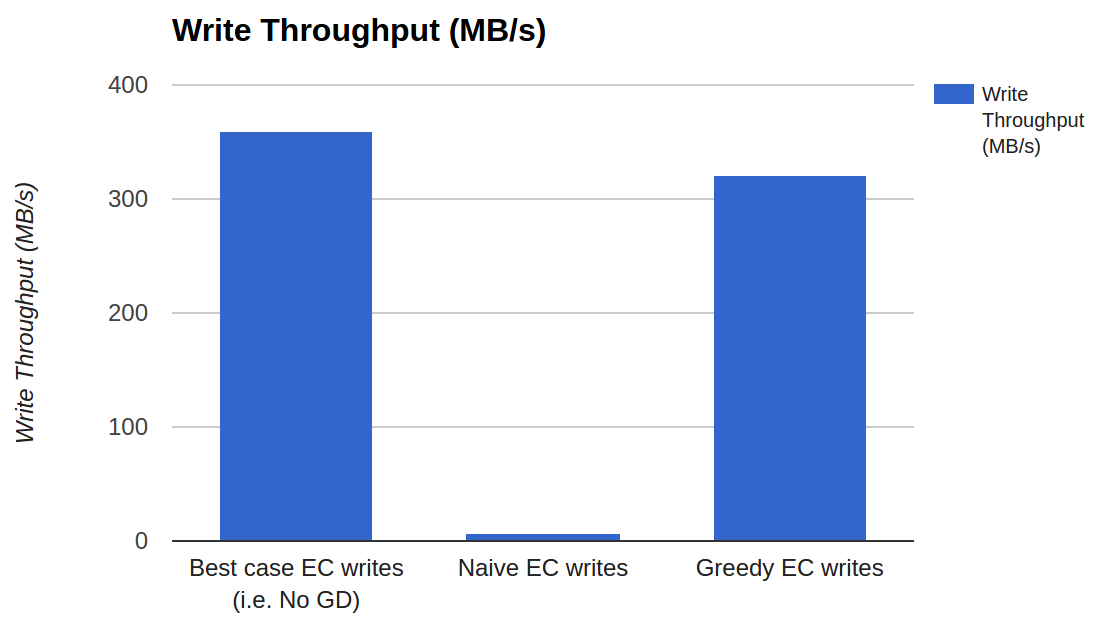
\includegraphics[scale=0.21]{greedy_write_tput.png}
\caption{HDFS-EC write throughput with No-GD (best case), Naive GD and Greedy WAN aware GD}
\label{greedyTput}
\end{figure} 

\begin{table}
\centering

\begin{tabular}{|c|c|c|c|l|} \hline
EC write type&Best case&Naive EC&Greedy EC\\ \hline
Throughput&359.81&7.26&321.42\\

\hline\end{tabular}
\caption{Results from greedy EC write tests}
\label{table:gd-writes}
\end{table}

\textbf{Results}: Figure \ref{greedyTput} and Table \ref{table:gd-writes} show the write throughputs observed in this setting. The \emph{Naive EC writes} bar represents the throughput observed when our greedy write algorithm is disabled. The \emph{Best case} bar represents the EC read speeds that were achieved in an intra-DC setting in \ref{sec:bench-results}. It acts as an upper bound to compare our greedy algorithm's performance. 

As can be seen, our greedy EC write algorithm achieves much higher throughput than a naive implementation in a GD setting. The naive approach ends up selecting a Utah node as one of the datanodes in order to meet its goal of rack fault tolerance. 

On the other hand, our greedy approach ends up selecting all the Wisconsin nodes for 5 datanodes because the WAN link cost is far greater than the \emph{sameRackPenalty}. It thus avoids using the WAN link altogether and achieves much higher performance.

The observed read throughput in the greedy case is also very close to the best case throughputs (ie. intra-DC throughputs). This proves that the minimal overhead of our greedy algorithm. 

\begin{figure}
\centering
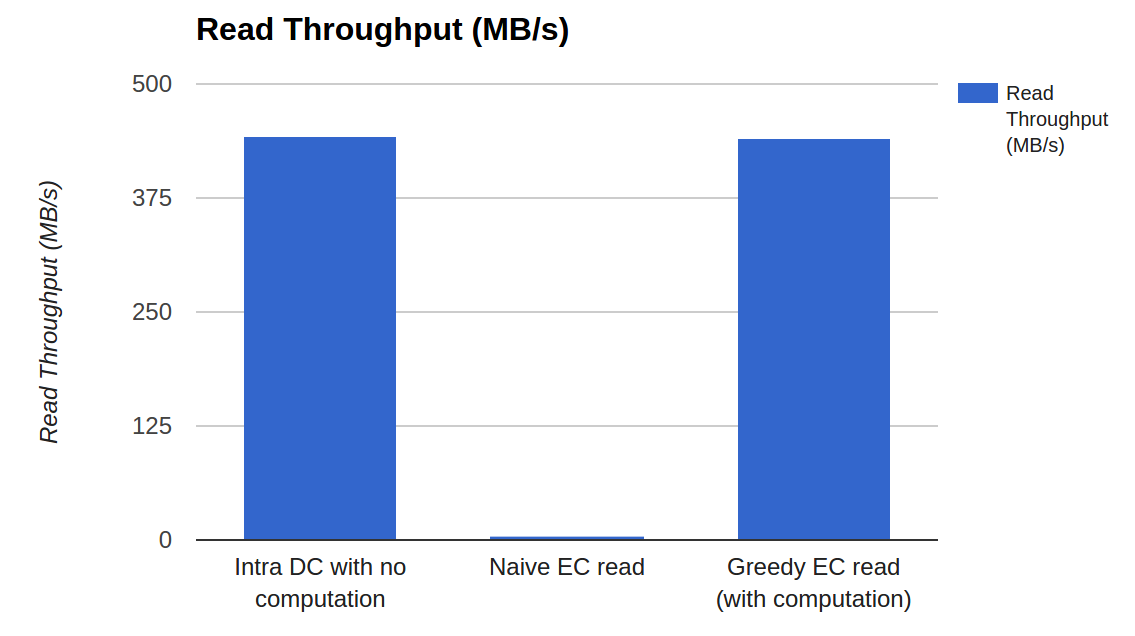
\includegraphics[scale=0.23]{greedy_read_tput.png}
\caption{HDFS-EC Read throughput with No-GD, Naive GD and Greedy WAN aware HDFS-EC-GD}
\label{greedyReadTput}
\end{figure} 

\begin{table}
\centering

\begin{tabular}{|c|c|c|c|l|} \hline
EC read type&Best case&Naive EC&Greedy EC\\ \hline
Throughput&442.53&4.61&439.67\\

\hline\end{tabular}
\caption{Results from greedy EC read tests}
\label{table:gd-reads}
\end{table}


\subsubsection{Greedy EC reads}
\textbf{Setup}: We reuse the setup from Section \ref{sec:greedy-ec-writes}. Only this time, we select a very high value for \emph{sameRackPenalty}, much higher than the WAN link cost. This results in data distribution similar to Figure \ref{gda-topo}, where one node in Utah holds data cells for a given file. The high value of \emph{sameRackPenalty} forces it to consider the Utah node early on because the WAN link cost is lower.

It is important to have the Utah node host data cells and not parity cells, because this would allow us to demonstrate the impact of our greedy EC read algorithm. We again run tests only for large files (ie. 1 GB). We pick 1 and 100 as the intra-DC and WAN link costs. We pick a parity \emph{computationalPenalty} of 10. \\

\textbf{Results}: Figure \ref{greedyReadTput} and Table \ref{table:gd-reads} show the results from our experiment. The \emph{Naive EC read} bar shows the read throughput achieved when our greedy behaviour is disabled. We again show the \emph{Best case EC read} figures as a useful tool for knowing the upper bound. 

As can be seen, our greedy EC read algorithm achieves much higher performance than a naive EC read implementation. The naive implementation would always prefer fetching the data cells unless they are lost. It will thus incur the penalty of using the WAN link in order to get the data cells from the Utah. 

On the other hand, our greedy algorithm correctly picks the parity cells available in Wisconsin nodes because the parity computation penalty is far lower than the WAN link cost. It is thus able to achieve much higher performance by bypassing the WAN link. 

\begin{figure}
\centering
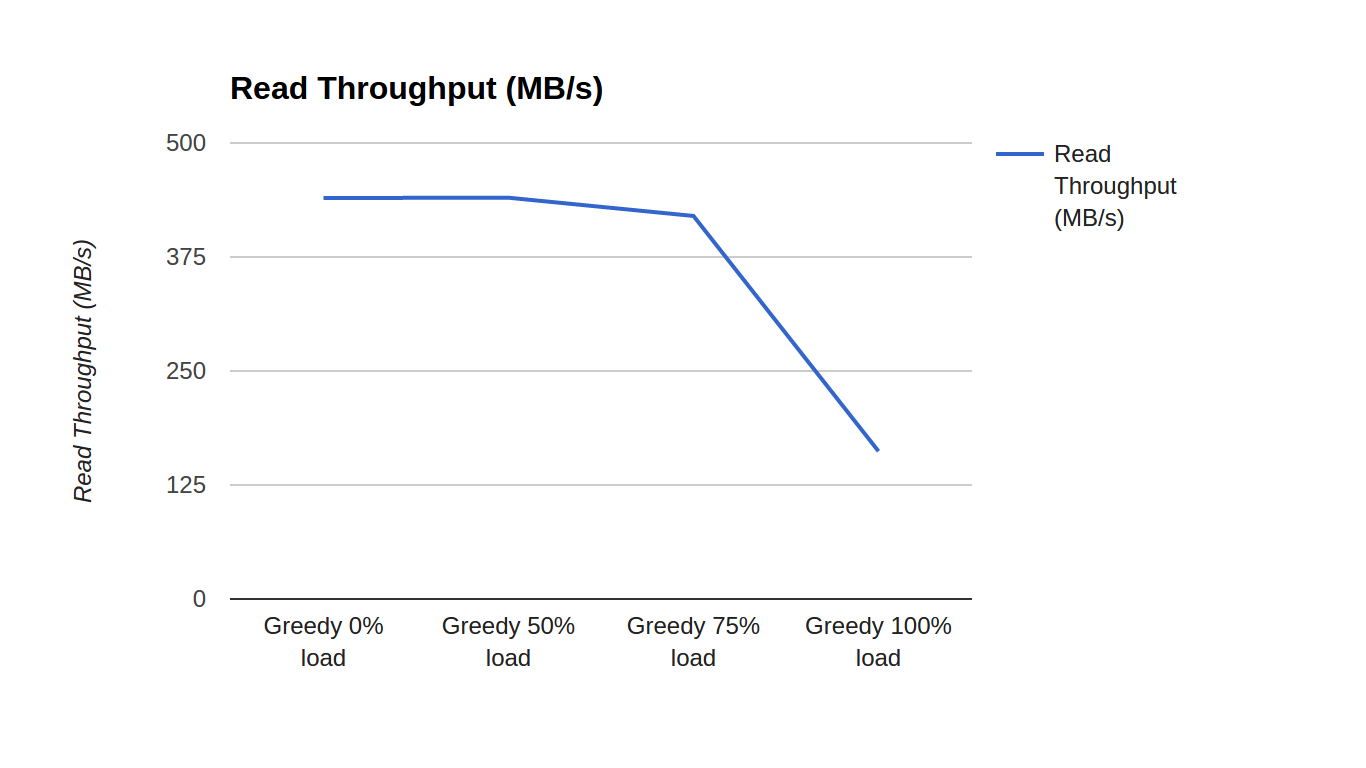
\includegraphics[scale=0.4]{stress.png}
\caption{Read throughput of greedy WAN aware HDFS-EC-GD with varying CPU load on all nodes}
\label{greedy-stress}
\end{figure}

\subsubsection{Impact of CPU load on parity computation}
A natural question which follows from our greedy EC read behaviour is -- how much is the overhead associated with doing parity computation? In order to find this out, we re-run our greedy EC read tests with varying CPU loads. We use the Linux \emph{stress} \cite{linux-stress} utility to generate CPU loads of 50\%, 75\% and 100\% on the namenode and all the datanodes. 

The results are shown in Figure \ref{greedy-stress}. The reduction in EC read performance is marginal -- about 5\% even when we have high CPU loads of 75\%. This shows the low CPU overhead and the efficiency of the ISA-L libraries used for encoding/decoding. These findings are also consistent with other studies, who have shown peak RS decoding throughputs of 1.8 GB/s using these libraries \cite{cloudera-blog}.

\section{Discussion}

\subsection{Erasure Coding Properties}

There are various kinds of encoding families that can be used to encode data. These include RS codes, LRC codes and the product codes. Since HDFS-EC used RS encoding, we will restrict our discussion to tradeoffs of using different values \emph{n} and \emph{k} in RS encoding. According to the coding theory an (n, k) RS code entails the minimum storage overhead among all (n, k) erasure codes that tolerate any \emph{k} failures \cite{hitchhiker}. Moreover, RS codes can be constructed with arbitrary values of \emph{n} and \emph{k} depending upon the system at hand \cite{hitchhiker}. These two properties make RS codes very attractive for use in large scale storage systems. 


The choice of the parameters \emph{n} and \emph{k} for any particular system determines the storage overhead and recovery cost for the system. In general achieving lower storage overhead increases the recovery cost of the system and vice versa. For Example, an RS(10, 4) system has a $1.4\times $ overhead compared to $1.5\times $ for RS (6, 3). However, in case of an unavailable datablock RS (10, 4) has to read 10 blocks while RS (6, 3) only needs to read 6.This trend can be generalized for any possible values or \emph{n} and \emph{k}. 



\subsection{Significance of Storage Unit to Encode}

The storage unit to be encoded is determined by the layout of the file system. This layout can be contiguous or striped. In contiguous layout a logical block of the file system is mapped directly to a datanode. Reading that block merely involves contacting that particular datanode and doing one I/O.  In striped block layout however, a single logical block in the file system is broken down into small cells and these cells are then mapped to the available datanodes in a round robin manner. Therefore, in the striped layout case, reading a single logical datablock of the file system involves doing I/O with all the datanodes that store the cells of that block. 

%This however, may not be very suitable for Map-Reduce style applications because data %locality cannot be achieved as most reads would involve multiple remote I/Os.

In the replication based storage, a contiguous layout seems to be an obvious choice as there is no point in paying an extra cost of many remote reads for every read event. However, in Erasure Coded storage, things become a little more interesting. This is because the number of parity blocks computed in RS encoding scheme is always equal to \emph{k} irrespective of the total number of data blocks in the file \cite{cloudera-blog}. For example, while using RS (10, 4) if a file consists of just one data block, it will still end up computing and writing 4 parity blocks resulting in a total storage overhead of 400\% which is worse than $3\times $ replication! However, in a striped layout and assuming a cell size of 1 MB and the HDFS data block size of 128MB the same 1 block file would still have a $1.4\times $ overhead since it will produce about 51 MBs of parity (since the parity is computed for 1 MB stripe cells) compared to 512 MB of parity produced by the contiguous layout for the same 128 MB file. 

Therefore, the type of file system layout directly affects the storage overhead for the erasure coding scheme at hand. This choice of layout in turn is determined the file size distribution on the cluster. Hence, a cluster with many small files is not suitable for erasure coding in the contiguous layout because the storage overhead would be worse than replication. The HDFS-EC alpha release that we used and extended uses a striped layout with 1 MB cell size. 

\section{Future Work}

Our greedy approaches for choosing datanodes for reads and writes show that they can be effective in reducing the performance degradation of HDFS running in GD settings. The benefits achieved by these schemes are due to the fact that they minimize the use of WAN in the read and write operations. 

However greedy heuristics are limited in their impact and can lead to other side effects. In our case, the greedy EC write approach can lead to data localization ie. data getting aggregated on a few local nodes leading to higher loads on them. The ideal solution would be to select datanodes based on solving a linear formulation based on several constraints. However we can not have the ILP solver in the critical path because it would slow down performance tremendously.

Instead, we can have a data movement process running as a background job, which solves this formulation and moves data around to satisfy several constraints. Since this is off the critical path, there are no issues. 

We can also create additional copies of data and parity cells based on some workload prediction. Several systems \cite{iridium}\cite{clarinet} have used this idea before. But none of them do it in a storage-efficient manner. We can perform this data copying in a bounded manner by trading off some of the storage benefits given by EC to achieve better performance. Eg. A customer could change his storage overhead from $1.5\times $ to $2\times $ and create extra copies of cells for improved GD performance.

Secondly, in the current implementation, the HDFS client reconstructs the data cells itself after reading one or more parity cells. This can be improved by performing reconstruction of data cells in parallel. We can have a coordinator node in each geo location and whenever an HDFS-EC-GD client prefers a local parity cell read over a remote data cell read, it can inform the coordinator node to initiate the parallel reconstruction of the data. This reconstruction job would be launched by the Coordinator node similar to a Map-Reduce job making sure that all the decoding workers write their output to the HDFS-EC-GD client node. This can dramatically speed up data reconstruction while also minimizing the effect of constrained cpu of the client itself. 

\section{Related Work}
Erasure coding is increasingly being preferred over replication to provide reliability in distributed file systems since it has a far smaller storage overhead. For example, Reed-Solomon \cite{RS} is a popular family of codes used in Google\textquotesingle s ColossusFS \cite{colossus}, Facebook\textquotesingle s HDFS \cite{hdfs-raid}, and several other storage systems \cite{rethink, hitchhiker, gpfs}
However erasure coding brings with itself higher block recovery costs. Multiple data blocks have to be brought in through the network to recompute one lost data block in erasure coding, whereas the corresponding network cost for in replication is just one block.  Several efforts have been made in trying to reduce the recovery cost by using alternate coding schemes - namely LRCs \cite{azure}, or using piggybacking mechanisms like in Hitchhiker\textquotesingle s \cite{hitchhiker}. One of the aims of our study is to find out how such strategies would need to be modified for a geo-distributed cluster setup. We can have a WAN-aware block picking strategy for block recovery, which will try to pick blocks nearby instead of over the WAN link.
There has also been some recent work on a hybrid storage system HACFS \cite{tale}, which uses two different erasure codes and dynamically adapts to workload changes. It uses a fast code to optimize for recovery performance and a compact code to reduce the storage overhead

\bibliographystyle{abbrv}
\bibliography{sigproc}

  \begin{thebibliography}{1}

  \bibitem{hitchhiker} J Rashmi, K. V., et al. "A hitchhiker\textquotesingle s guide to fast and efficient data reconstruction in erasure-coded data centers." ACM SIGCOMM Computer Communication Review. Vol. 44. No. 4. ACM, 2014.

  \bibitem{cloudera-blog}  http://blog.cloudera.com/blog/2015/09/introduction-to-hdfs-erasure-coding-in-apache-hadoop/
  
  \bibitem{hdfs-ec} https://hadoop.apache.org/docs/r3.0.0-alpha1/hadoop-project-dist/hadoop-hdfs/HDFSErasureCoding.html

  \bibitem{tale}Xia, Mingyuan, et al. "A tale of two erasure codes in hdfs." 13th USENIX Conference on File and Storage Technologies (FAST 15). 2015.
  
  \bibitem{RS} REED, AND SOLOMON - Polynomial codes over certain finite fields. Journal of the So-ciety for Industrial and Applied Mathematics.
  
  \bibitem{colossus} Colossus, successor to Google File System.
  
  \bibitem{hdfs-raid} Facebook\textquotesingle s erasure coded hadoop distributed file system (HDFS-RAID). 
  
  \bibitem{rethink} KHAN, BURNS, PLANK, PIERCE, AND HUANG - Rethinking erasure codes for
cloud file systems: Minimizing I/O for recovery and degraded reads.

  \bibitem{gpfs} SCHMUCK, AND HASKIN - GPFS: A shared-disk file system for large computing clusters. 
  
  \bibitem{azure} HUANG, SIMITCI, XU, OGUS, CA, IDER, GOPALAN, LI, YEKHANI - Erasure coding in Windows Azure Storage
  
  \bibitem{iridium} PU, ANANTHANARAYANAN, BODIK, KANDULA, AKELLA, BAHL, AND STOICA - Low Latency Geo-distributed Data Analytics
  
  \bibitem{clarinet} VISWANATHAN, ANANTHANARAYANAN, AND AKELLA - Clarinet: WAN-Aware Optimization for Analytics Queries
  
  \bibitem{isa-l} Intel ISA-L: https://github.com/01org/isa-l
  
  \bibitem{linux-stress} Linux stress tool - https://linux.die.net/man/1/stress
  

  \end{thebibliography}



\end{document}
